\documentclass[11pt]{article}
\usepackage[margin=1in]{geometry}
\usepackage{amsmath,amssymb}
\usepackage{graphicx}
\usepackage{booktabs}
\usepackage[colorlinks=true,linkcolor=blue,citecolor=blue,urlcolor=blue]{hyperref}

% --- the only two lines to edit before submission ---
\newcommand{\authorname}{Singularity}
\newcommand{\affiliation}{}

\title{Kolmogorov--Arnold layers inside an Energy Flow Network\\ for quark/gluon jet tagging}
\author{\authorname\\ \small \affiliation}
\date{\today}

\begin{document}
\maketitle

\begin{abstract}
Energy Flow Networks (EFNs) classify jets by summing a learned per-particle function weighted by momentum fraction.
We replace the multilayer perceptrons of a compact EFN with Kolmogorov--Arnold (spline) layers, keeping inputs,
summation and parameter count fixed, and test it on public simulated light-quark and gluon jets. In a pilot with
200,000 training jets and three seeds, the KAN version raised the test AUC from 0.8306 to 0.8584 (paired 95\% interval
for the difference $+0.0266$ to $+0.0293$), with gains on a second Pythia file and on Herwig jets. A full-scale check,
fixed in advance, trained on 1.6 million jets and compared the KAN EFN (2,239 parameters) with a wider standard EFN of
13,025 parameters: the KAN version was still better on the new primary file, AUC 0.8665 against 0.8573 (difference
$+0.0091$, interval $+0.0081$ to $+0.0100$), and on all three other test files, including two from a different
generator. At 80\% quark efficiency the gluon mistag rate fell from 24.9\% to 22.6\%, with a network six times
smaller.
\end{abstract}

\section{Introduction}
An EFN~\cite{efn} maps each jet constituent through a learned function of its angular coordinates, sums the outputs
weighted by the constituent's momentum fraction, and classifies the resulting latent observables with a second
network. The construction is infrared and collinear safe. Kolmogorov--Arnold networks~\cite{kan} replace fixed
activations with learned one-dimensional splines and can represent smooth functions with few parameters. KAN-inspired
geometric networks have already been tried on quark/gluon tagging~\cite{gkan}; the question here is narrower: inside
the same EFN structure, with the same inputs and a matched parameter budget, do spline layers separate quark and
gluon jets better than perceptrons?

\section{Methods}
\paragraph{Data.} Pythia light-quark and gluon jets~\cite{pythiadata} (20 files of 100,000 jets) and Herwig jets of
the same selection~\cite{herwigdata} for transfer without retraining. Inputs are constituent rapidity and azimuth
relative to the jet axis and normalised transverse-momentum weights.
\paragraph{Models.} All models share the EFN sum with 16 latent observables. EFN MLP: perceptron encoder and head
(2,209 parameters). EFN KAN: spline layers in encoder and head (2,239). Spline + MLP: spline encoder with a perceptron
head (2,041), to isolate the encoder. For the spline encoder the momentum-weighted sum of basis functions is linear
and is precomputed exactly. Numerical checks on centred inputs confirm the expected symmetries: maximum logit change
$7.2\times10^{-6}$ under particle permutation, $5.6\times10^{-6}$ under collinear splitting and $2.0\times10^{-5}$ under
soft emission.
\paragraph{Pilot.} 200,000 training and 100,000 validation jets; three seeds per model, six epochs, checkpoint chosen
by validation AUC; predictions averaged over seeds. Test files: Pythia 18 (primary), Pythia 19 (replica, already
present in an earlier exploratory folder) and Herwig 1. Criterion: AUC gain of at least 0.003 on the primary file, a
paired bootstrap interval above zero, and positive mean-over-seeds gains on both other files.
\paragraph{Full scale.} Fixed in writing before training: all 20 Pythia files, split by file into 1.6 million training
jets (files 0--15), 200,000 validation (18--19, already seen in the pilot) and 200,000 new test jets (16 primary, 17
replica), plus 200,000 Herwig jets (files 2--3). The main comparator is a wide EFN with $64\times64$ encoder and head
and 32 latent observables (13,025 parameters); the compact EFN is secondary. Five full passes, seed 17, AdamW,
batch 1,024, learning rate 0.002 with cosine decay, checkpoint by mean validation AUC, no tuning on test files. Same
criterion as the pilot, with positive differences required on all three non-primary files. Intervals resample jets and
are conditional on the trained models.

\section{Results}
\begin{table}[h]
\centering
\begin{tabular}{lrrrr}
\toprule
test file & EFN KAN & wide EFN & compact EFN & KAN $-$ wide [95\% interval] \\
\midrule
Pythia 16 (primary) & \textbf{0.86646} & 0.85734 & 0.84659 & $+0.00912$ [0.00813, 0.00995] \\
Pythia 17 & 0.86589 & 0.85754 & 0.84579 & $+0.00835$ [0.00744, 0.00924] \\
Herwig 2 & 0.79713 & 0.78998 & 0.78125 & $+0.00715$ [0.00599, 0.00833] \\
Herwig 3 & 0.79854 & 0.79099 & 0.78242 & $+0.00756$ [0.00646, 0.00864] \\
\bottomrule
\end{tabular}
\caption{Full-scale test AUC (1.6 million training jets). Parameters: KAN 2,239; wide EFN 13,025; compact EFN 2,209.}
\label{tab:full}
\end{table}

\begin{table}[h]
\centering
\begin{tabular}{lrrr}
\toprule
test file & EFN MLP & EFN KAN & spline + MLP \\
\midrule
Pythia 18 (primary) & 0.83060 & \textbf{0.85838} & 0.84553 \\
Pythia 19 & 0.83093 & 0.85996 & 0.84627 \\
Herwig 1 & 0.77519 & 0.79502 & 0.78448 \\
\bottomrule
\end{tabular}
\caption{Pilot test AUC (200,000 training jets, three-seed ensembles, matched parameter counts).}
\label{tab:pilot}
\end{table}

\begin{figure}[h]
\centering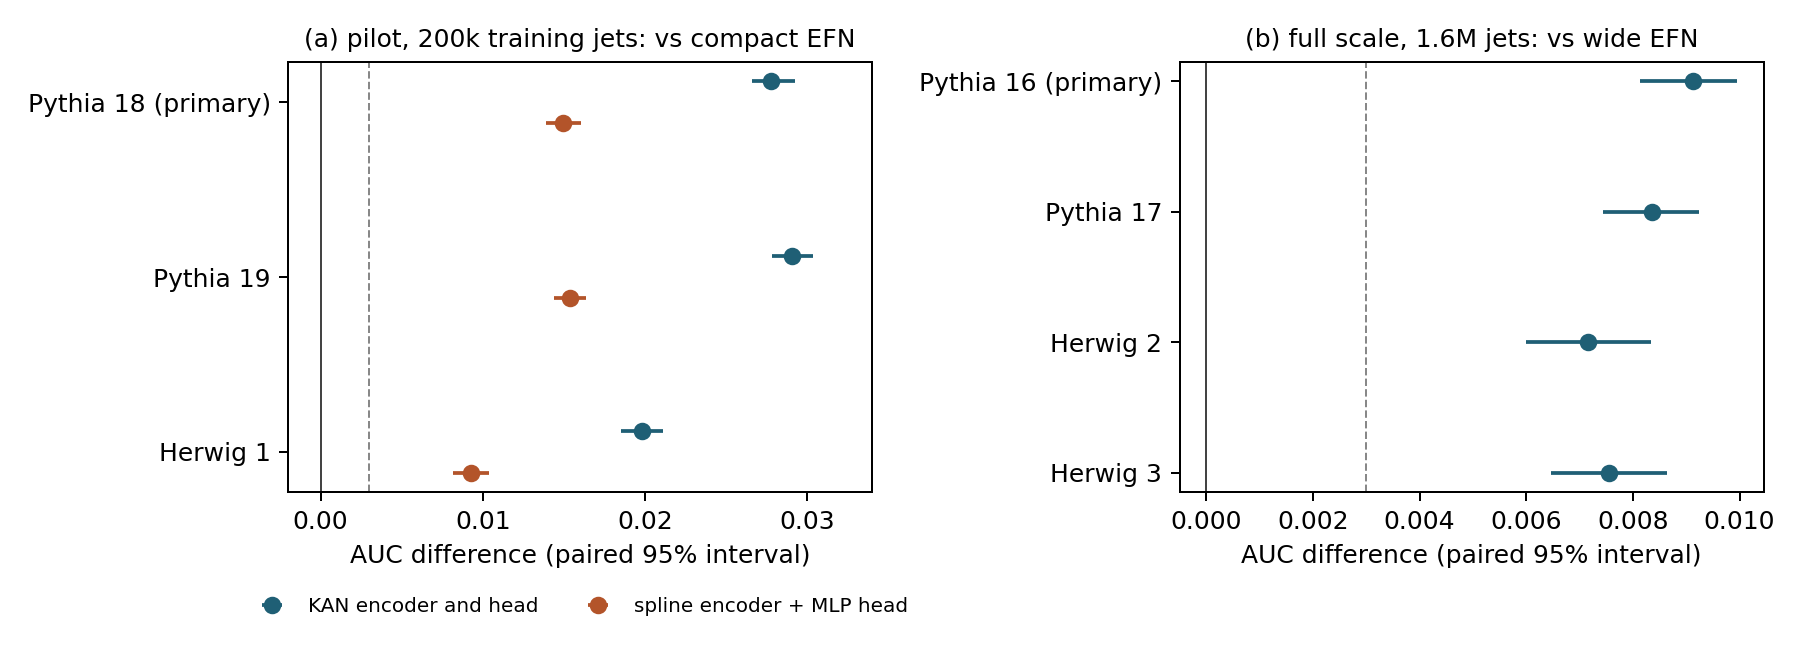
\includegraphics[width=\linewidth]{fig_results.png}
\caption{AUC differences with paired 95\% intervals. Dashed line: the pre-specified minimum gain of 0.003.}
\label{fig:results}
\end{figure}

\begin{itemize}
\item \textbf{Pilot.} The KAN EFN met the criterion: $+0.0278$ on the primary file (interval $+0.0266$ to
$+0.0293$), $+0.0290$ on Pythia 19 and $+0.0198$ on Herwig. The spline encoder alone recovered about half of the gain.
\item \textbf{Not only undertraining.} With 16 epochs and one seed the gap narrowed but remained: 0.8610 against 0.8432
on the primary file and 0.7951 against 0.7826 on Herwig.
\item \textbf{Full scale.} With eight times more training data and against a perceptron EFN with six times more
parameters, the KAN EFN still met the criterion on all four test files (Table~\ref{tab:full}).
\item \textbf{Working point.} At 80\% quark efficiency the gluon mistag rate on the primary file was 22.6\% (KAN),
24.9\% (wide EFN) and 27.6\% (compact EFN).
\end{itemize}

\section{Discussion}
Learned one-dimensional splines appear to be a good fit for the per-particle function of an EFN, which is a smooth
map of two angular coordinates, and for the head, which acts on a small number of latent observables. The advantage
shrinks from about 0.028 to 0.009 in AUC when the comparator is larger and better trained, which is the more relevant
figure for practice; it persists across generators, so it is not specific to Pythia's modelling of the jets. Since
the swap keeps the EFN's safety properties and parameter budget, it is a cheap change to try in other jet-tagging
tasks and with detector-level simulation.

\paragraph{Limitations.} Simulated jets in one transverse-momentum range from two generators, without detector
effects. The full-scale comparison uses one training run per architecture; in the pilot the KAN was also the more
stable across seeds (0.854 to 0.857, against 0.813 to 0.838 for the compact perceptron EFN).

\paragraph{Reproducibility.} \texttt{experiment.py} runs, in order, the pilot, the 16-epoch sensitivity check, the
full-scale preparation, training of the three networks, evaluation and the figure. \texttt{results.json}
contains the pilot metrics per seed and ensemble, the sensitivity check and the full-scale metrics; trained weights and
validation curves are in \texttt{code/results/}.

\paragraph{Origin of the question.} The question came from an automated forecast (Singularity v2, registered on 2
November 2026 with a SHA-256 fingerprint) that Kolmogorov--Arnold networks would enter experimental high-energy
physics. The forecast concerned the arrival of the method, not the result of this study.

\begin{thebibliography}{9}
\bibitem{efn} P.~T.~Komiske, E.~M.~Metodiev and J.~Thaler, Energy flow networks: deep sets for particle jets,
\emph{JHEP} 01 (2019) 121, arXiv:1810.05165.
\bibitem{kan} Z.~Liu et al., KAN: Kolmogorov--Arnold networks, arXiv:2404.19756 (2024).
\bibitem{gkan} F.~Alesiani et al., Geometric Kolmogorov--Arnold superposition theorem, arXiv:2502.16664 (2025).
\bibitem{pythiadata} P.~T.~Komiske, E.~M.~Metodiev and J.~Thaler, Pythia 8 quark and gluon jets for energy flow,
Zenodo (2019), doi:10.5281/zenodo.3164691.
\bibitem{herwigdata} P.~T.~Komiske et al., Herwig 7.1 quark and gluon jets, Zenodo (2019),
doi:10.5281/zenodo.3066475.
\end{thebibliography}
\end{document}
